\appendix
\section{Planner comparison}
\label{app:planners}

We compare four planners offline on the 110 ordered start/station pairs from the route-planning benchmark (11 points: three starts and eight observation cells). Dijkstra and A* are the controller's own implementations; greedy best-first search (GBFS) orders the frontier by the Manhattan heuristic alone; turn-penalised A* searches over (cell, heading) with cost $=$ cells $+\,w\cdot$turns, $w=1$, since a $90^\circ$ turn takes about as long as driving one cell. Timing is the median of 25 repeats on one CPU core. We checked all 440 paths for validity (adjacent free cells, consistent move labels).

\begin{table*}[tbp]
  \centering\small
  \setlength{\tabcolsep}{3pt}
  \begin{tabular}{@{}lccccc@{}}
    \toprule
    Planner & ms & vs.\ Dijkstra & Optimal & Length ratio & Turns \\
            & (median) & (speed-up) & pairs & mean / max & total (mean) \\
    \midrule
    Dijkstra              & 0.637 & 1.0$\times$  & 110/110 & 1.000 / 1.00 & 308 (2.8) \\
    A* (final)            & 0.127 & 4.2$\times$  & 110/110 & 1.000 / 1.00 & 324 (2.9) \\
    GBFS                  & 0.060 & 10.3$\times$ & 84/110  & 1.059 / 2.29 & 383 (3.5) \\
    A* + turn penalty     & 0.450 & 1.2$\times$  & 110/110 & 1.000 / 1.00 & 170 (1.5) \\
    \bottomrule
  \end{tabular}
  \caption{Offline planner comparison on all 110 ordered start/station pairs (median time of 25 repeats on one CPU core; path length relative to the Dijkstra optimum; turns are heading changes along the path). Optimality matters (GBFS is longer on 26 pairs), planning speed does not (all under 1\,ms), and turn count is the cost that remains to optimise.}
  \label{tab:planners}
\end{table*}

\Cref{tab:planners} shows three things. First, optimality matters: GBFS is the fastest planner but returns a longer path on 26 of 110 pairs, up to $2.29\times$ the optimum, and needs 18\% more turns than A*. Second, A* and Dijkstra give paths of identical length; A*'s $4.2\times$ speed-up is real but irrelevant to mission time, because every query finishes in under a millisecond. Third, the metric that does affect mission time is the number of turns. Among equally short paths, the turn-penalised variant needs 47\% fewer turns than A* (170 vs.\ 324). It is not used in the submitted controller and is left as future work (\cref{sec:discussion}).

\section{Full encoder comparison}
\label{app:encoders}

\Cref{fig:headline} extends \cref{tab:encoders} to every method of the encoder study, with simulated mission success as a third metric.

\begin{figure*}[tbp]
  \centering
  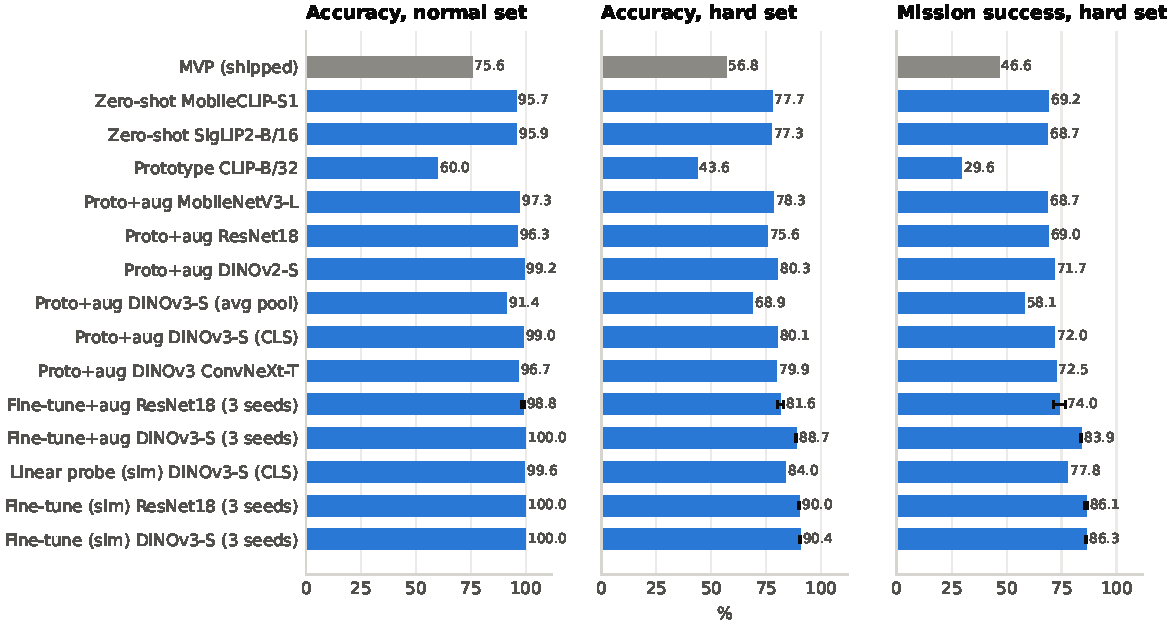
\includegraphics[width=\textwidth]{figs/p_headline.pdf}
  \caption{Accuracy on the normal and hard capture sets and simulated mission success (random station order, stop at the first positive, success if that station is correct) for every method, measured on frames from stations the method never saw; fine-tune bars show the mean and s.d.\ of 3 seeds. Training-free DINOv3 prototypes already beat the first detector by 23 points on the hard set, and fine-tuning DINOv3 on the eight references gives the best accuracy (88.7\%) and mission success (83.9\%) without any simulator data.}
  \label{fig:headline}
\end{figure*}

\section{Development history}
\label{app:git}

\begin{figure*}[tbp]
  \centering
  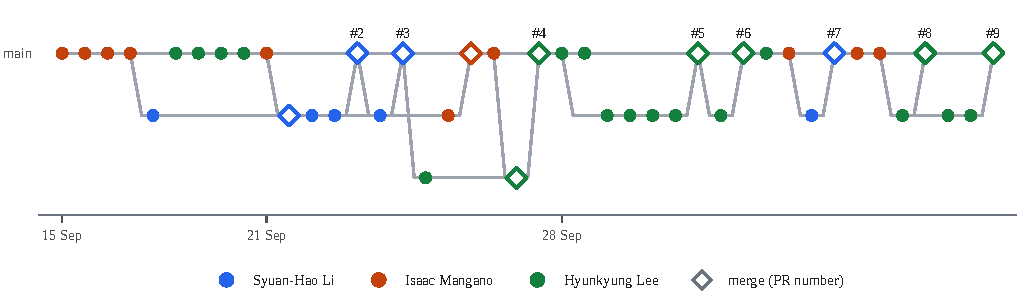
\includegraphics[width=\textwidth]{figs/git_graph.pdf}
  \caption{Commit graph of the shared repository up to the final controller (42 commits, plotted in topological order with a weekly date axis): the main line, the feature branches and the pull-request merges (diamonds, numbered), with each commit coloured by its author. Work from all three members entered the main line through branches and pull requests, continuously across the three weeks. Some of Isaac's commits appear on a side lane because they arrived through a sync from his upstream repository.}
  \label{fig:git}
\end{figure*}

